\begin{figure}[H]
\caption{The Haar functions}\label{figure:haar}
\centering
\caption*{\\[1em]\footnotesize\textit{(a) The Haar wavelet function (mother
wavelet)}}
\[
\begin{aligned}
\Psi(t) = \left\{
	\begin{array}{r r}
		1  & \quad   0 \leq t < 1/2, \\
		-1 & \quad 1/2 \leq t < 1, \\
		0  & \quad \text{otherwise.}
	\end{array}
\right.
\end{aligned}
\qquad
\raisebox{-15mm}{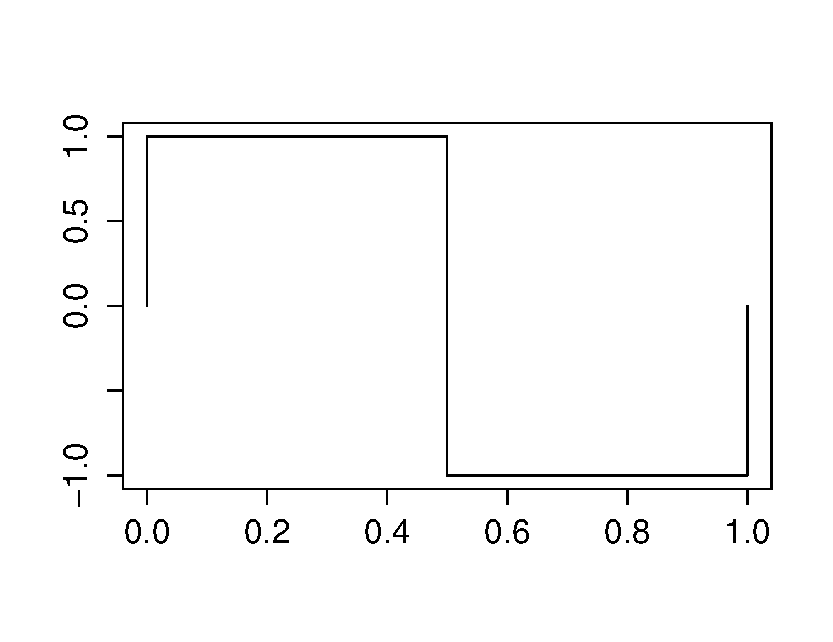
\includegraphics[height=128pt]{images/haar.pdf}}
\]
\caption*{\footnotesize\textit{(b) The Haar scaling function (father wavelet)}}
\[
\Phi(t) = \left\{
	\begin{array}{r r}
		1 & \quad 0 \leq t < 1, \\
		0 & \quad \text{otherwise.}
	\end{array}
\right.
\]
\end{figure}
